\documentclass[11pt,a4paper]{article}

% ------------------------------------------------
% Packages
% ------------------------------------------------
\usepackage[utf8]{inputenc}
\usepackage[T1]{fontenc}
\usepackage[a4paper, margin=1in]{geometry}
\usepackage{graphicx}
\usepackage{float}
\usepackage{booktabs}
\usepackage{setspace}
\usepackage{parskip}
\usepackage{titlesec}
\usepackage{xcolor}
\usepackage{caption}
\usepackage{hyperref}
\usepackage{listings}
\usepackage{xcolor}

\definecolor{codebg}{rgb}{0.97,0.97,0.97}
\definecolor{codecomment}{rgb}{0.0,0.45,0.0}
\definecolor{codekeyword}{rgb}{0.1,0.1,0.65}
\definecolor{codestring}{rgb}{0.58,0,0.82}

\lstdefinestyle{rcode}{
	language=R,
	backgroundcolor=\color{codebg},
	basicstyle=\ttfamily\small,
	keywordstyle=\color{codekeyword}\bfseries,
	commentstyle=\color{codecomment},
	stringstyle=\color{codestring},
	numbers=left,
	numberstyle=\tiny,
	stepnumber=1,
	numbersep=8pt,
	breaklines=true,
	breakatwhitespace=false,
	showstringspaces=false,
	frame=single,
	tabsize=2,
	captionpos=b
}
% ------------------------------------------------
% Formatting
% ------------------------------------------------
\setstretch{1.15}
\setlength{\parindent}{0pt}
\setlength{\parskip}{0.7em}

\hypersetup{
	colorlinks=true,
	linkcolor=black,
	urlcolor=blue,
	citecolor=black
}

\titleformat{\section}
{\large\bfseries}
{\thesection.}{0.5em}{}

\titleformat{\subsection}
{\normalsize\bfseries}
{\thesubsection}{0.5em}{}

\captionsetup{
	font=small,
	labelfont=bf
}

% ------------------------------------------------
% Title info
% ------------------------------------------------
\title{\textbf{Data Visualisation for Social Scientists\\Final Project Report}}
\author{Qi Liu}
\date{March 2026}

% ------------------------------------------------
% Document
% ------------------------------------------------
\begin{document}
	
	\maketitle
	\thispagestyle{empty}
	
	\tableofcontents
	\newpage
	
	\vspace{1em}
	
\section*{Executive Summary}
\addcontentsline{toc}{section}{Executive Summary}
	
	This project examines neighbourhood-level air quality in New York City, focusing on two pollutants (NO2 and PM2.5) around 2017. The goal is to tell a concise data story about (i) where pollution is most concentrated, (ii) how much seasonal averages differ from annual averages, and (iii) whether neighbourhoods face a ``co-burden'' across pollutants. After filtering the dataset to mean values for three comparable time windows (Winter 2016--17, Summer 2017, Annual average 2017), the analytic sample includes 141 neighbourhoods observed for both pollutants in all three periods (846 observations in total). Across four figures, I show that pollution burdens are spatially concentrated in a small set of neighbourhoods, seasonal patterns differ by pollutant, and NO2 and PM2.5 tend to move together across neighbourhoods---suggesting that some places face layered exposure risks that annual averages can partially conceal.
	
	\section*{Data Background}
	\addcontentsline{toc}{section}{Data Background}
	
	The dataset reports air quality indicators by geographic unit (``Geo Place Name'') and reporting window (``Time Period''). Each row corresponds to one indicator measurement for a specific neighbourhood and time period, with the outcome recorded as ``Data Value'' (mean concentration in the pollutant's unit). For this project, I focus on Indicator ID 375 (NO2) and Indicator ID 365 (PM2.5), because they are widely discussed urban pollutants and are both available at neighbourhood scale in the dataset. I centre the analysis on 2017 and use three comparable summaries---Winter (2016--17), Summer (2017), and Annual average (2017)---to make seasonal contrasts interpretable while keeping the story coherent.
	
\section*{Data Cleaning}
\addcontentsline{toc}{section}{Data Cleaning}

I began with the full dataset (18,862 rows, 12 columns) and restricted attention to measurements that can be meaningfully compared across neighbourhoods and time. Specifically, I filtered to \texttt{Measure == "Mean"}, selected only NO2 (Indicator ID 375) and PM2.5 (Indicator ID 365), and kept only three time periods: Winter (2016--17), Summer (2017), and Annual average (2017). I then converted \texttt{Data Value} to a numeric variable, removed rows with missing or non-numeric values, and created cleaner labels for both pollutants and time periods. This step ensures that the later visualisations compare like with like across neighbourhoods and seasons. The final cleaned dataset is balanced by design: 141 neighbourhoods $\times$ 2 pollutants $\times$ 3 time periods (846 observations).

To make the cleaning process transparent, the key R code is shown below.

\begin{lstlisting}[style=rcode, caption={Key R code for data cleaning and variable preparation}]
	# Load data
	aq_raw <- readxl::read_excel(file.path("data", "Air_Quality.xlsx"))
	
	# Define pollutants and time periods of interest
	ID_PM25 <- 365
	ID_NO2  <- 375
	
	TP_ANNUAL <- "Annual Average 2017"
	TP_SUMMER <- "Summer 2017"
	TP_WINTER <- "Winter 2016-17"
	
	keep_tp <- c(TP_ANNUAL, TP_SUMMER, TP_WINTER)
	
	# Filter and clean data
	aq <- aq_raw %>%
	filter(Measure == "Mean") %>%
	filter(`Indicator ID` %in% c(ID_PM25, ID_NO2)) %>%
	filter(`Time Period` %in% keep_tp) %>%
	mutate(
	`Data Value` = suppressWarnings(as.numeric(`Data Value`)),
	indicator = case_when(
	`Indicator ID` == ID_PM25 ~ "PM2.5",
	`Indicator ID` == ID_NO2  ~ "NO2",
	TRUE ~ "Other"
	),
	time_period = factor(
	`Time Period`,
	levels = c(TP_WINTER, TP_SUMMER, TP_ANNUAL),
	labels = c("Winter (2016--17)", "Summer (2017)", "Annual avg (2017)")
	),
	place = `Geo Place Name`
	) %>%
	filter(!is.na(`Data Value`))
\end{lstlisting}

After cleaning, the resulting dataset provides a consistent neighbourhood-level panel for comparing pollutant levels across seasons and annual averages. This cleaned structure directly supports the four figures that follow.
	
	\section*{Individual Figures}
	\addcontentsline{toc}{section}{Individual Figures}
	
    \subsection*{Figure 1: Lollipop Chart}
    \addcontentsline{toc}{subsection}{Figure 1: Lollipop Chart}
	
	First, I wanted to find out which neighbourhoods had the worst pollution levels in 2017, because citywide averages can hide the fact that some places are much more affected than others. I therefore used a lollipop chart to rank neighbourhoods by their annual average level for each pollutant. The figure shows that the highest values are grouped in a relatively small number of areas, with several of them located in central Manhattan, such as Midtown, the Upper East Side, Gramercy Park–Murray Hill, and the Financial District/Lower Manhattan. So even at the annual level, pollution does not seem to be evenly distributed across neighbourhoods. To make the chart easier to read, I only show the top 12 neighbourhoods for each pollutant.
	
	\begin{lstlisting}[style=rcode, caption={Key R code for Figure 1: lollipop chart of top neighbourhoods}]
		TOP_N <- 12
		
		aq_annual <- aq %>%
		filter(time_period == "Annual avg (2017)") %>%
		group_by(indicator, place) %>%
		summarise(value = mean(`Data Value`), .groups = "drop")
		
		top_places <- aq_annual %>%
		group_by(indicator) %>%
		slice_max(order_by = value, n = TOP_N, with_ties = FALSE) %>%
		ungroup()
		
		p1 <- top_places %>%
		mutate(place = fct_reorder(place, value)) %>%
		ggplot(aes(x = value, y = place)) +
		geom_segment(aes(x = 0, xend = value, y = place, yend = place)) +
		geom_point(size = 2) +
		facet_wrap(~ indicator, scales = "free_x") +
		labs(
		title = "Figure 1. Highest-pollution neighbourhoods (Annual average 2017)",
		x = "Mean concentration (units differ by pollutant)",
		y = NULL,
		caption = "Ranking based on Annual average 2017."
		) +
		theme_minimal(base_size = 11)
	\end{lstlisting}
	
	\begin{figure}[H]
		\centering
		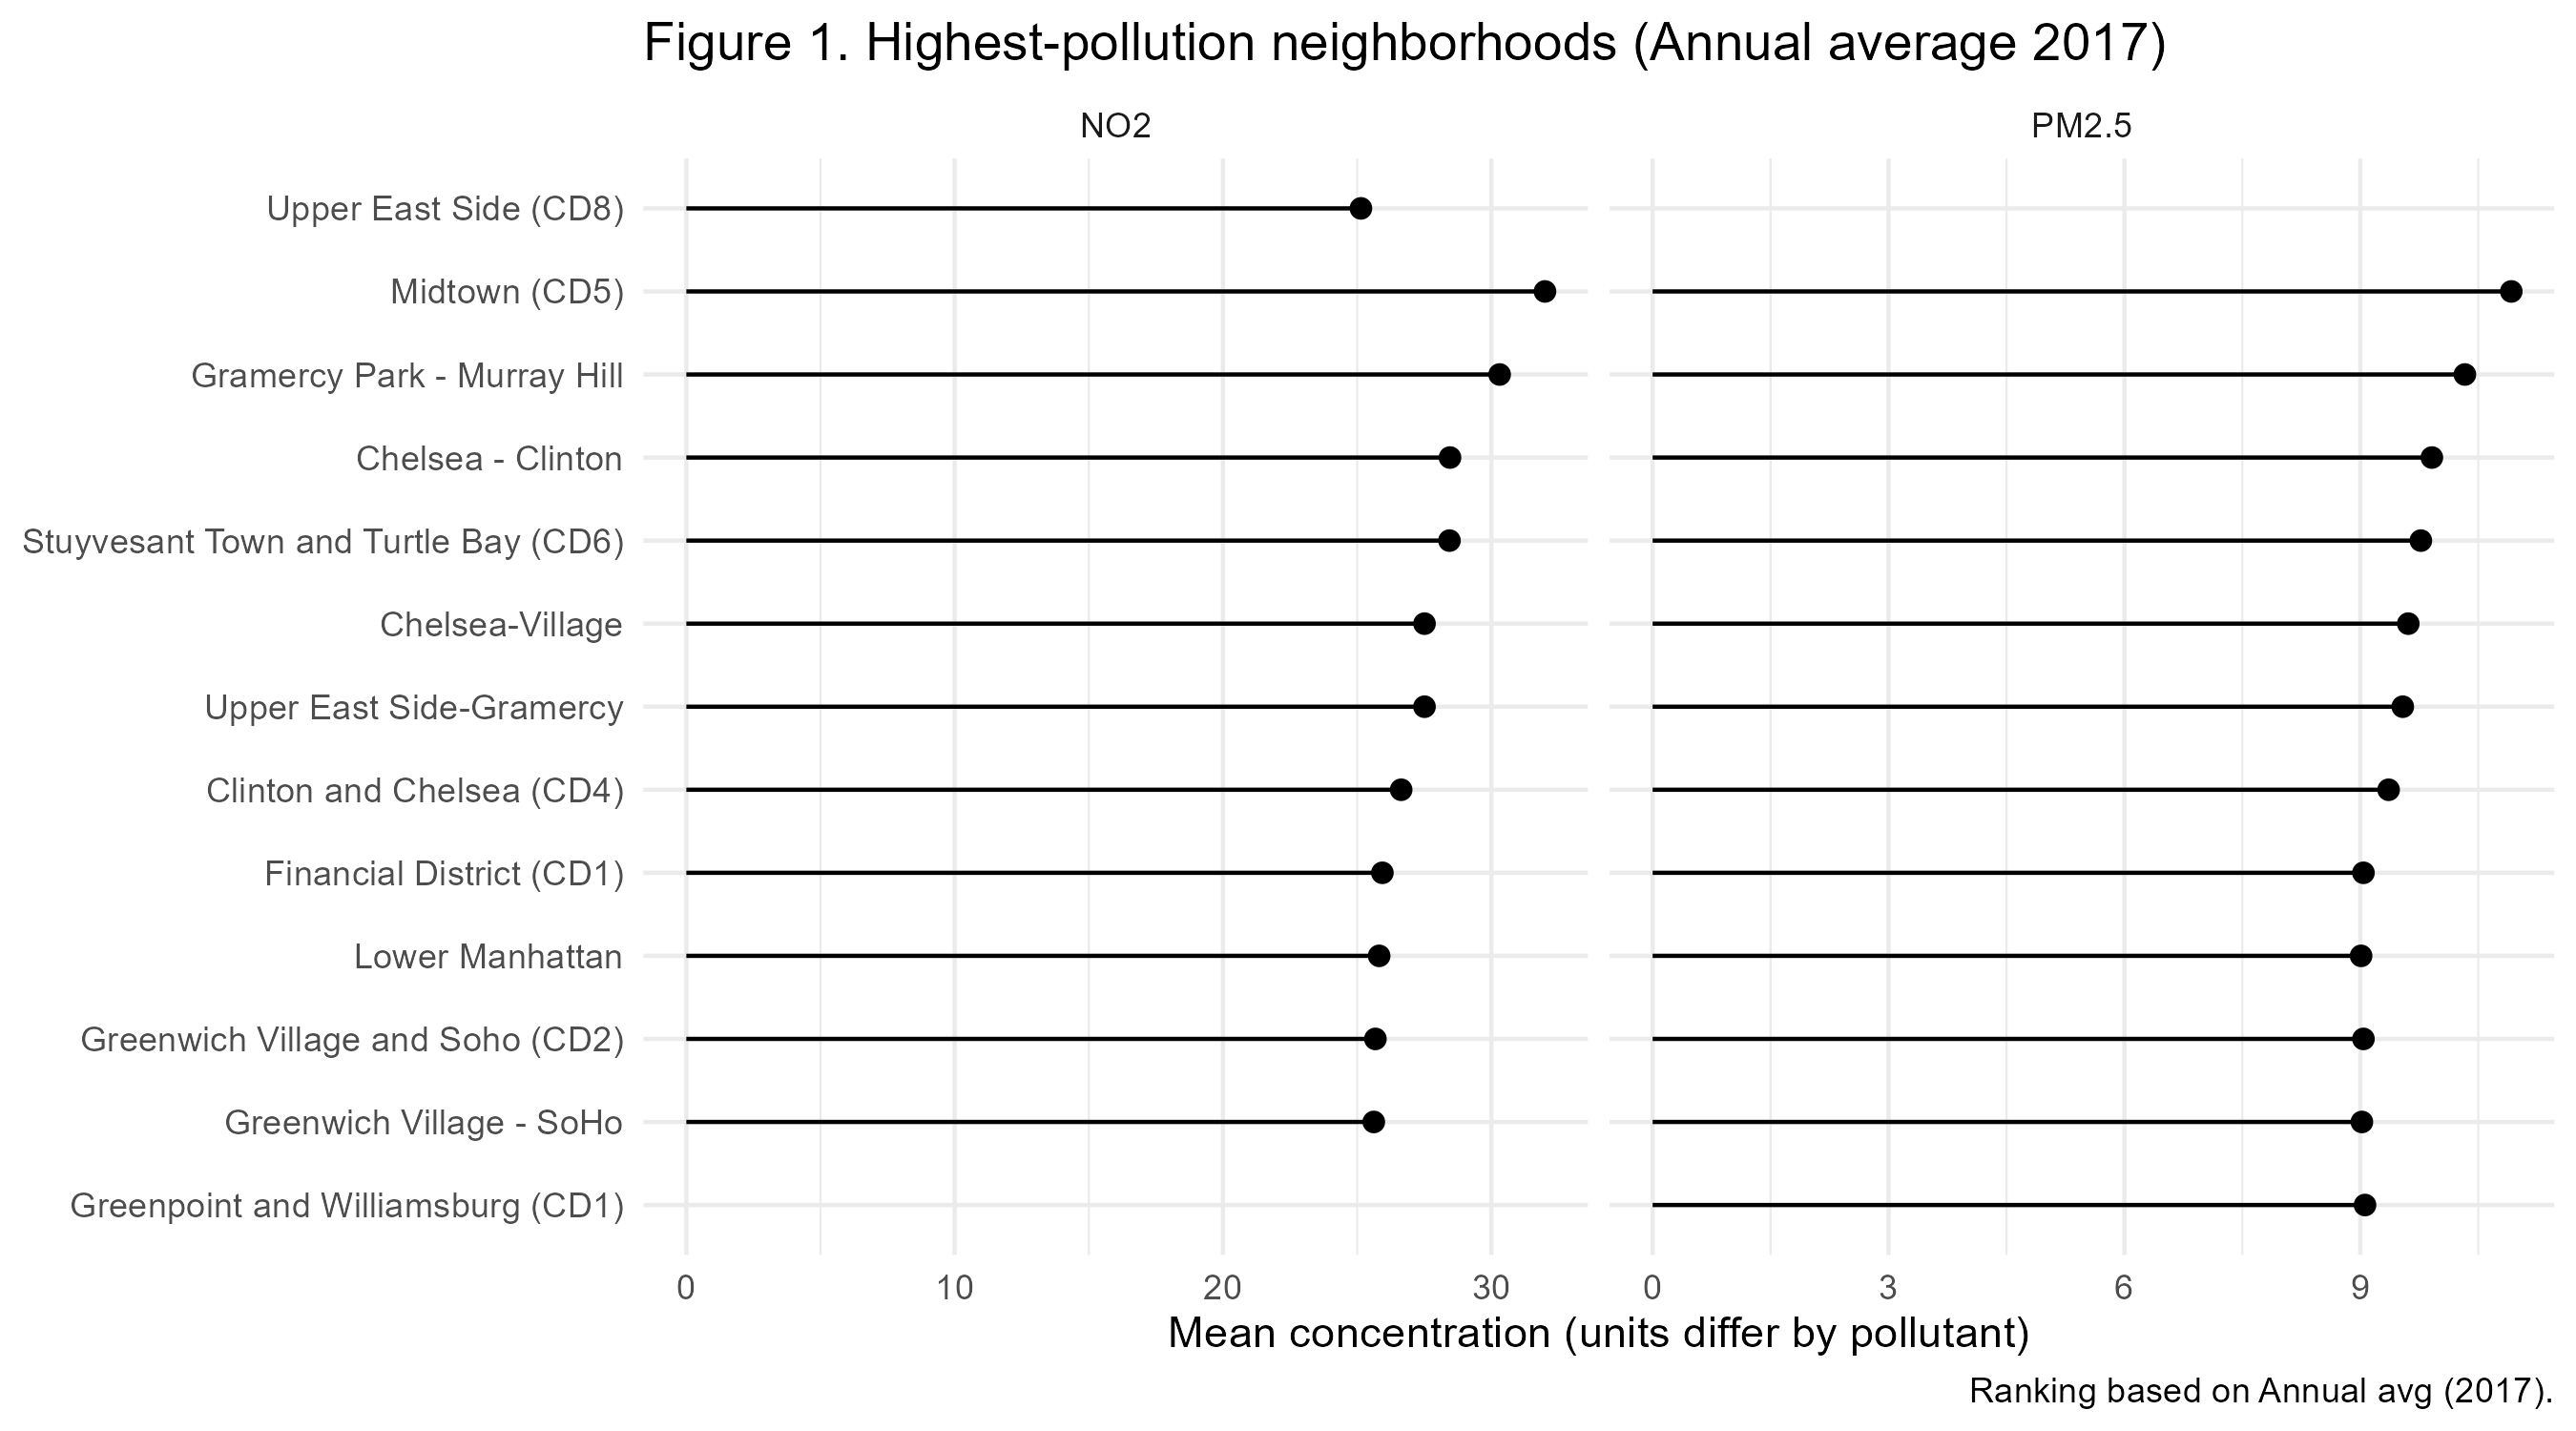
\includegraphics[width=0.95\textwidth]{figures/fig1_lollipop_top_neighborhoods_annual2017.png}
		\caption{Highest-pollution neighbourhoods, annual average 2017.}
	\end{figure}
	
	\subsection*{Figure 2: Boxplot}
	\addcontentsline{toc}{subsection}{Figure 2: Boxplot}
	
	Next, I wanted to check whether annual averages hide important seasonal differences, since pollution can be much worse at certain times of the year. To explore this, I used boxplots to compare the distributions across neighbourhoods in Winter (2016–17), Summer (2017), and the Annual average (2017). The figure shows clear seasonal patterns, but the direction differs by pollutant. NO2 is generally higher in winter and lower in summer, while PM2.5 shows the opposite pattern and tends to be higher in summer. In most cases, the annual average falls between the two seasonal values, which suggests that annual summaries can hide periods when exposure is especially high. Overall, this supports looking at seasonal patterns directly instead of relying only on a single yearly measure.
	
\begin{lstlisting}[style=rcode, caption={Key R code for Figure 2: boxplots by time period}]
	p2 <- aq %>%
	ggplot(aes(x = time_period, y = `Data Value`)) +
	geom_boxplot(outlier.alpha = 0.3) +
	facet_wrap(~ indicator, scales = "free_y") +
	labs(
	title = "Figure 2. Seasonal versus annual distributions",
	x = NULL,
	y = "Mean concentration (units differ by pollutant)",
	caption = "Annual averages may hide seasonal peaks and tail risk."
	) +
	theme_minimal(base_size = 11) +
	theme(axis.text.x = element_text(angle = 15, hjust = 1))
\end{lstlisting}
	
	\begin{figure}[H]
		\centering
		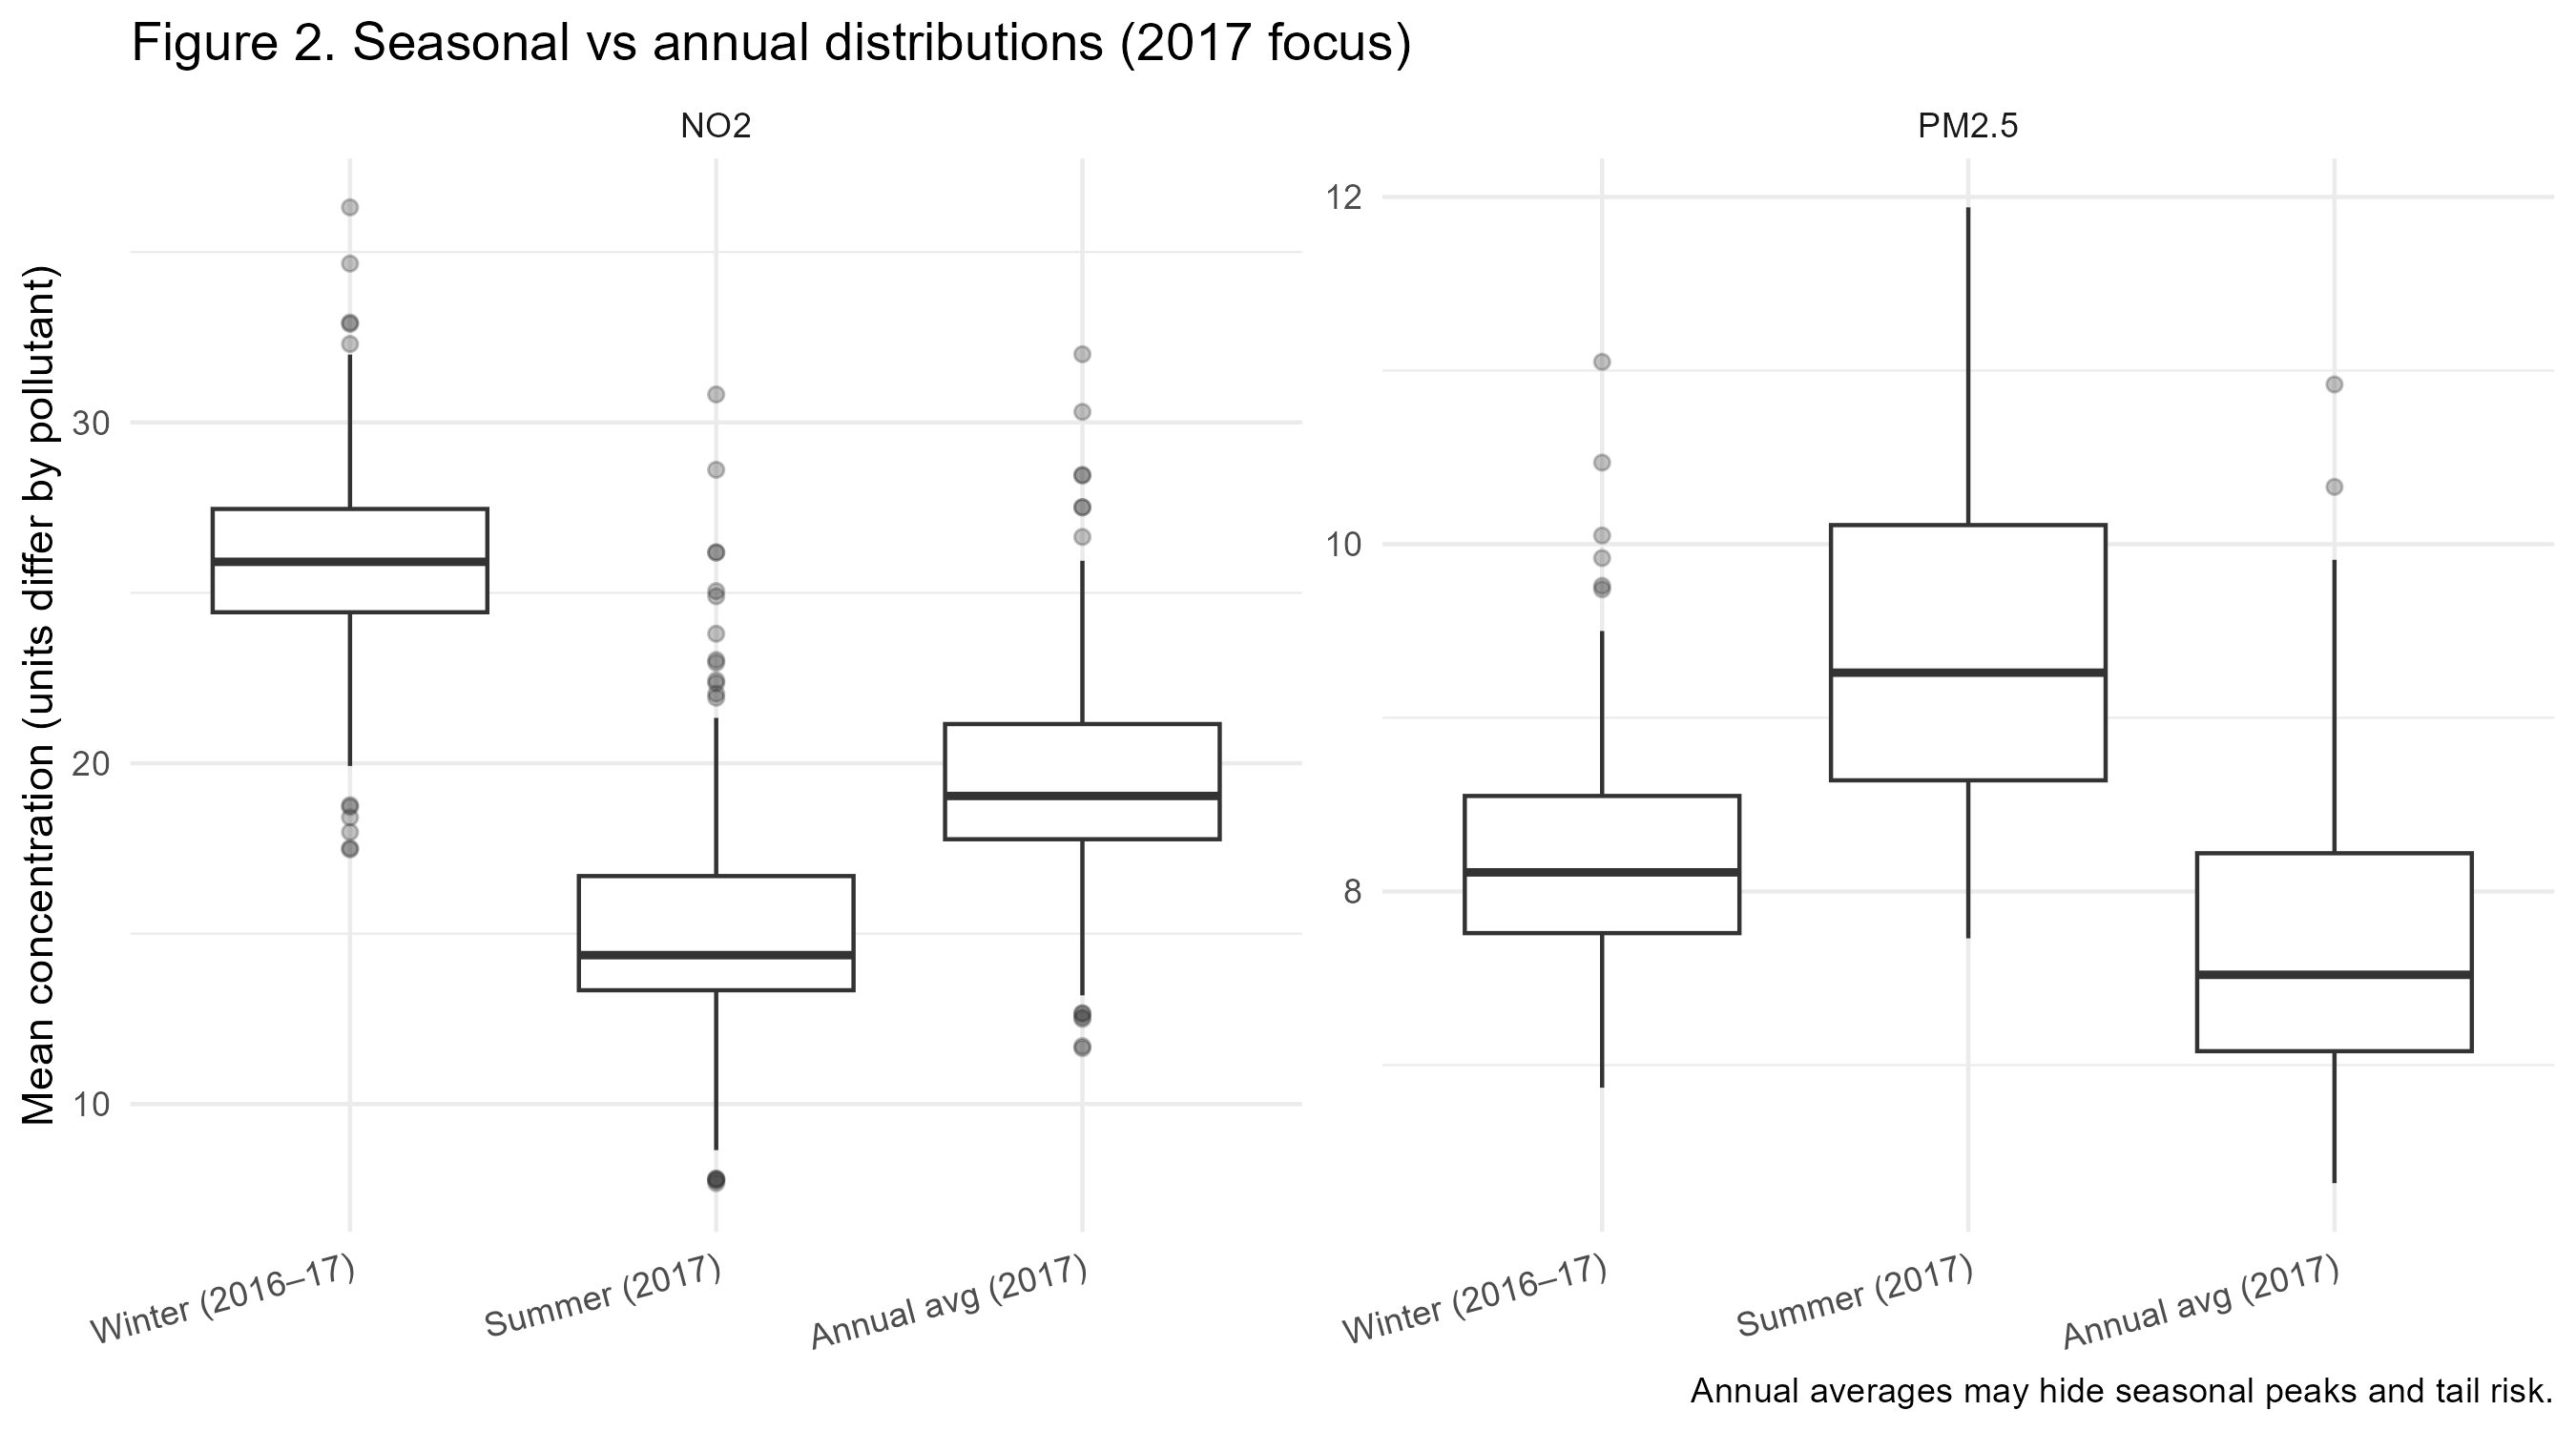
\includegraphics[width=0.95\textwidth]{figures/fig2_boxplot_distribution_by_period.png}
		\caption{Seasonal versus annual distributions across neighbourhoods.}
	\end{figure}
	
	\subsection*{Figure 3: Scatterplot of Relationships}
	\addcontentsline{toc}{subsection}{Figure 3: Scatterplot of Relationships}
	
	I was also interested in whether neighbourhoods with higher NO2 tended to have higher PM2.5, since that would mean some places face a combined pollution burden rather than just one type of pollutant. To look at this, I made a scatterplot of PM2.5 against NO2 for each time period. Across winter, summer, and the annual average, the relationship is generally positive, so neighbourhoods with higher NO2 also tend to have higher PM2.5. At the same time, the points do not all fall tightly around the fitted line, which suggests that the two pollutants do not affect neighbourhoods in exactly the same way. This is only a descriptive pattern, but it helps show that the main pollution hotspots often overlap across pollutants.
	
	\begin{lstlisting}[style=rcode, caption={Key R code for Figure 3: relationship between NO2 and PM2.5}]
		aq_wide <- aq %>%
		group_by(time_period, indicator, place) %>%
		summarise(value = mean(`Data Value`), .groups = "drop") %>%
		pivot_wider(names_from = indicator, values_from = value) %>%
		filter(!is.na(NO2), !is.na(`PM2.5`))
		
		p3 <- aq_wide %>%
		ggplot(aes(x = NO2, y = `PM2.5`)) +
		geom_point(alpha = 0.5) +
		geom_smooth(method = "lm", se = FALSE) +
		facet_wrap(~ time_period) +
		labs(
		title = "Figure 3. Relationship between NO2 and PM2.5",
		x = "NO2 (ppb)",
		y = "PM2.5 (mcg/m3)",
		caption = "Descriptive relationship only; line shows linear fit."
		) +
		theme_minimal(base_size = 11)
	\end{lstlisting}
	
	\begin{figure}[H]
		\centering
		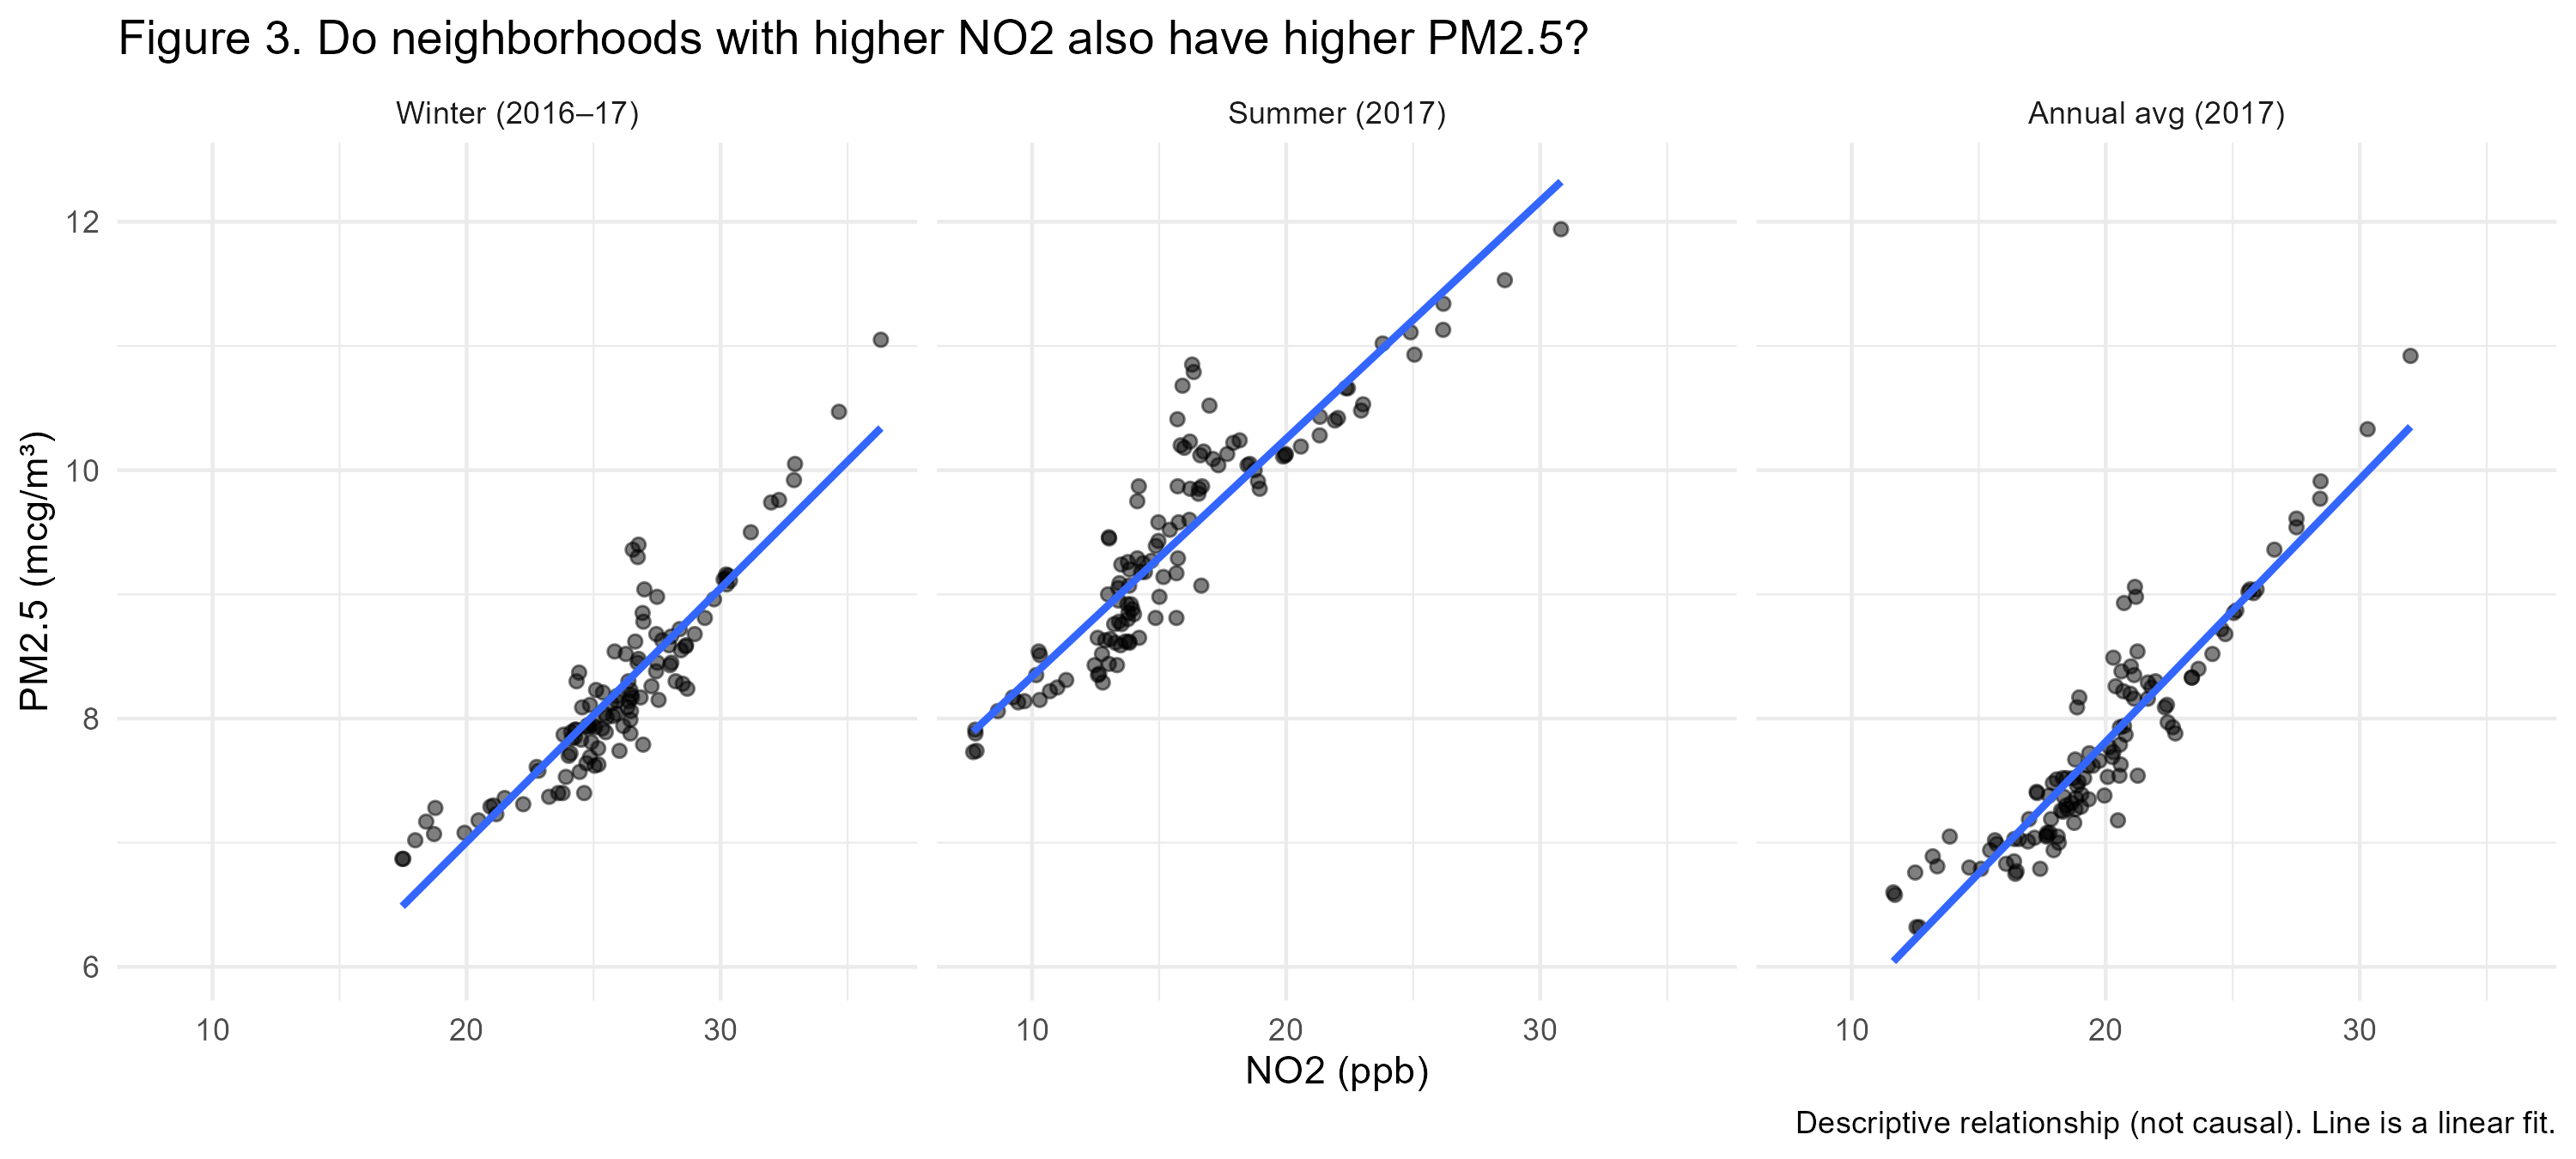
\includegraphics[width=0.98\textwidth]{figures/fig3_scatter_relationship_by_period.png}
		\caption{Relationship between NO2 and PM2.5 across neighbourhoods by time period.}
	\end{figure}
	
	\subsection*{Figure 4: Paired Seasonal Shift}
	\addcontentsline{toc}{subsection}{Figure 4: Paired Seasonal Shift}
	
	Finally, I wanted to see where seasonal differences were largest, because the change between winter and summer might be much bigger in some neighbourhoods than in others. To examine this, I used a paired plot comparing Winter (2016–17) and Summer (2017) for the neighbourhoods with the biggest seasonal changes. For NO2, the selected neighbourhoods show a clear increase from summer to winter. For PM2.5, the pattern goes in the opposite direction, with values generally higher in summer and lower in winter. This shows that seasonal peaks differ by pollutant, so the period with the highest exposure is not the same for NO2 and PM2.5. In other words, the size of the seasonal change is not the same across all neighbourhoods.
	
\begin{lstlisting}[style=rcode, caption={Key R code for seasonal shift plot}]
	season_delta <- aq %>%
	filter(time_period %in% c("Winter (2016-17)", "Summer (2017)")) %>%
	group_by(indicator, place, time_period) %>%
	summarise(value = mean(`Data Value`), .groups = "drop") %>%
	pivot_wider(names_from = time_period, values_from = value) %>%
	mutate(delta = `Winter (2016-17)` - `Summer (2017)`)
	
	delta_long <- season_delta %>%
	select(indicator, place, `Winter (2016-17)`, `Summer (2017)`) %>%
	pivot_longer(
	cols = c(`Winter (2016-17)`, `Summer (2017)`),
	names_to = "season",
	values_to = "value"
	)
\end{lstlisting}
	
	
	\begin{figure}[H]
		\centering
		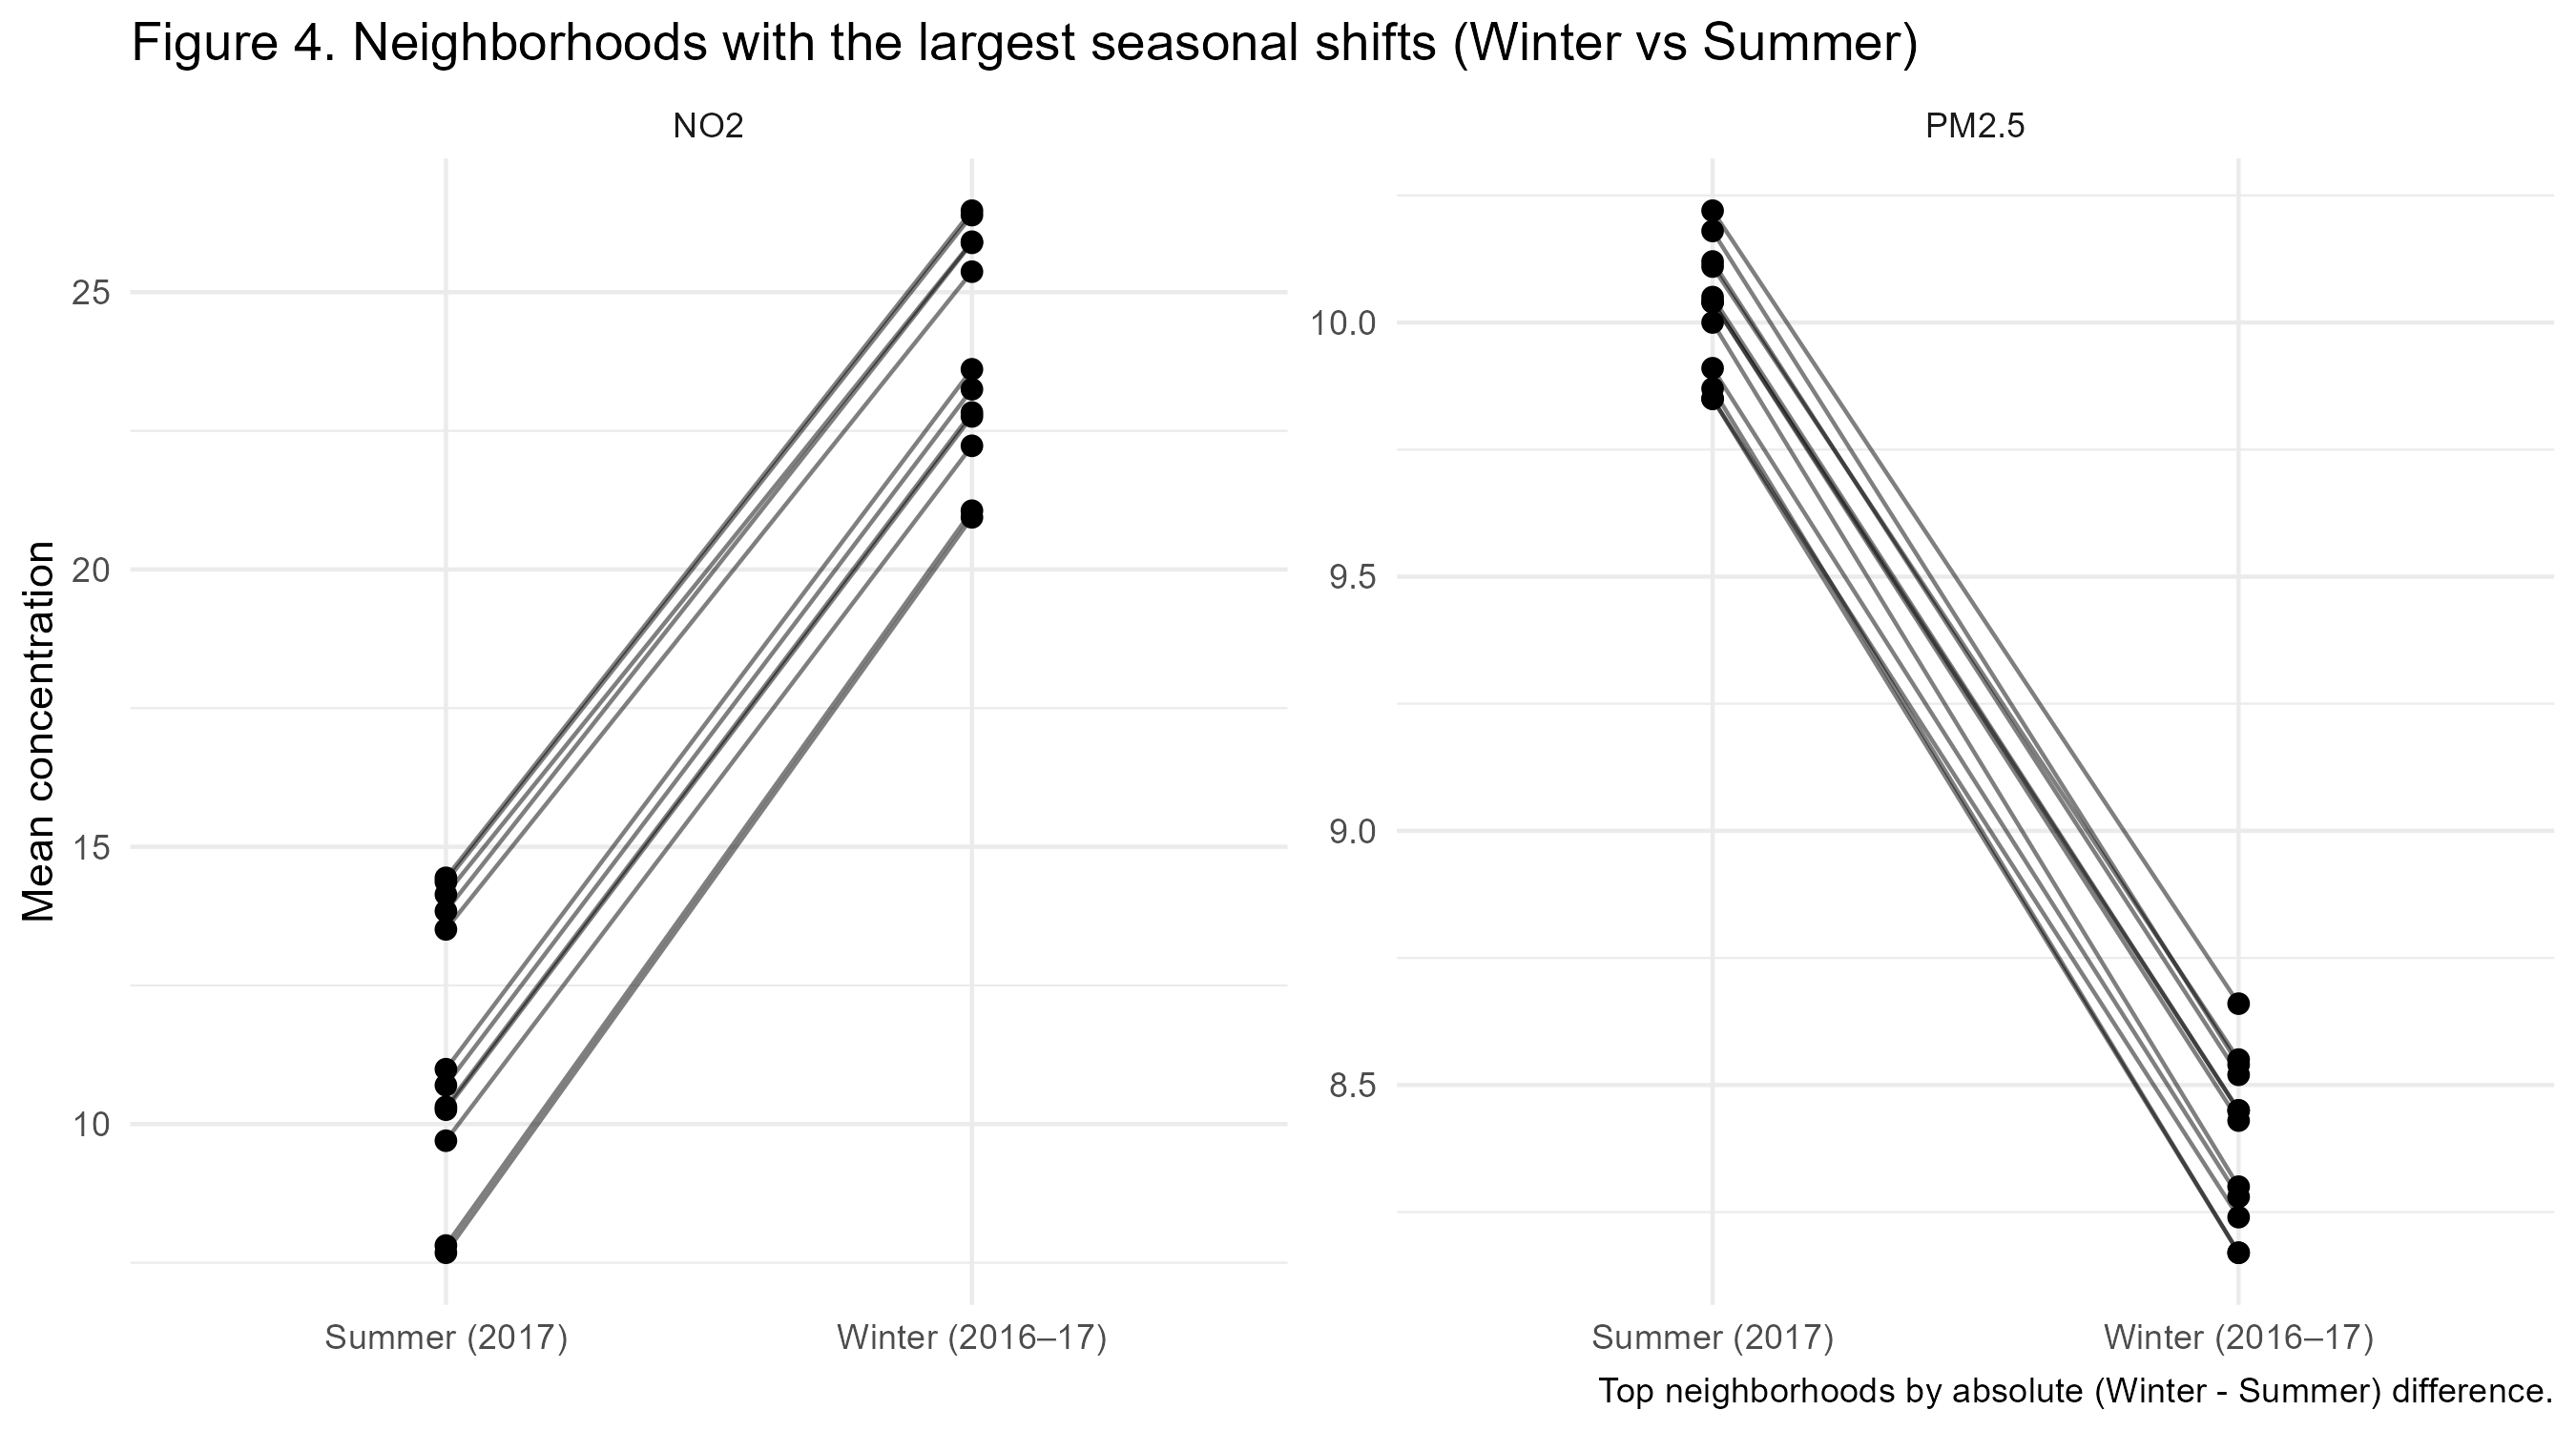
\includegraphics[width=0.95\textwidth]{figures/fig4_paired_seasonal_shift.png}
		\caption{Neighbourhoods with the largest seasonal shifts between winter and summer.}
	\end{figure}
	
\end{document}